\chapter{Softare Structure}
\label{Structure}

\par This software is comprised of several interconnected modules.  Each module represents an abstract concept required for modelling a traffic scenario, each containing as many classes as are needed to create the components necessarily for that concept.  This results in the creation of three self\-contained modules representing the network, the cars/objects traversing the network, and the state-changer.  To make the simulation complete and fully self-contained, the user may utilize two additional optional modules for generating the network structure and car objects. Following normal naming conventions, and module that a user may directly interact with has been named using capitalization; dependent modules (hidden to the user) are named using only lowercase.

\section{Essential Modules for the Network Traffic Simulator}

\subsection{Network Module:  traffic\_network}

\par As noted in the previous chapter, a network must have three components (network structure, nodes, and edges) \textit{and} there exists an inherent hierarchy to these structures (a network only exists by defining sets of connected nodes).  Though for creation purposes it may make sense to define the nodes and edges and let the network be a dependent object, that does not make sense for the problem at hand:  traffic simulation is the analysis of objects moving over a network, therefore the Network itself must be given (requiring a class of its own), leading to Nodes and Edges being dependent classes.  The module \textbf{traffic\_network} has been created to collect the instances and interactions of all network components for a simulation instance.  \\

\par The resulting module structure is as follows:

\begin{figure}[H]
    \centering
	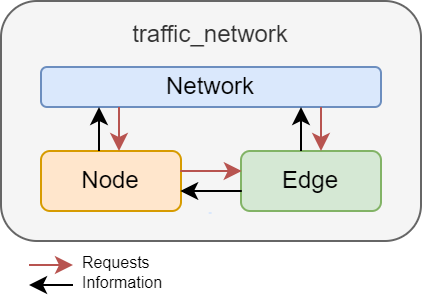
\includegraphics[width=0.5\textwidth]{tex files/Figures/traffic_network_module.png}
	\caption[Network Module:  traffic\_network]{Hierarchical structure of classes within the traffic\_network module.  Directions of requests and information flow between classes is depicted by colored arrows }
	\label{fig:network_module}
\end{figure}


\subsection{Car Module:  network\_cars}

\par "Car" is the general term I use to describe an object traversing the network as it allows for intuitive labeling of its attributes.  Once instantiated, a car is not dependent on the network to continue existing; to represent this semi-independence, the Car class was moved to a separate module:

\begin{figure}[H]
    \centering
	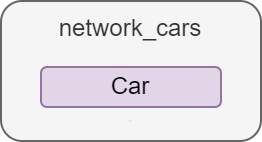
\includegraphics[width=0.3\textwidth]{tex files/Figures/car_module.png}
	\caption[Car Module:  network\_cars]{Classes structure within the network\_cars module}
	\label{fig:cars_module}
\end{figure}

\par In practice, though, the car is not very interesting when trying to simulate overall network behavior and ensuing traffic scenarios.  Any attributes the user may care about (such as current location) are only relevant in context.  So while \textbf{network\_cars} technically exists as a self-contained module, it is never used in isolation.  Instead, this module is automatically imported into the \textbf{traffic\_network} module, seamlessly allowing these two modules to interact with one another.


\subsection{State Module:  Traffic}

\par The final component necessary to creating a simulation  is a mechanism for advancing the state of the network.  State changing includes adding, removing, and advancing any cars on the network as far as possible within a particular unit of time, and are all essential for creating a hands-off simulation. \\

\par But simulation state refers to more than the set of current car locations.  It includes system metadata (like lists of nodes and edges in a network, and their attributes) and dependent calculations from that metadata.  By allowing the user an access point to adapt any component of the network, this software achieves its goal of being adaptable and extensible to other types of networks and simulations.  \\

\par The Traffic modules serves as an API to the underlying simulation, allowing users to (indirectly) interact with the network components and car objects.  The set of all these access points into the simulation allows for the direct management of traffic and has thus been wrapped into an aptly named class,  \textbf{TrafficManager}:

\begin{figure}[H]
    \centering
	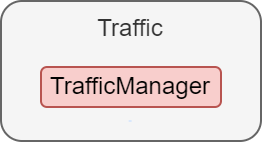
\includegraphics[width=0.3\textwidth]{tex files/Figures/traffic_manager_module.png}
	\caption[State Module:  Traffic\_cars]{Classes structure within the Traffic module}
	\label{fig:traffic_module}
\end{figure}


\noindent  Note that the \textbf{Traffic} module allows only for indirect access to the simulation components.  By using this API as an intermediary between users and network simulation components, the user is given access only to commands that are relevant to analysis, and hide internal functions that facilitate those actions.  For example, if a user wants a particular car to halt in place, they can call on the API function that requests it.  The \textbf{Traffic} module then passes that request to the \textbf{traffic\_network} and/or \textbf{network\_cars} module to handle if and when it becomes relevant.


\section{Essential Module Interaction}

\par Putting the modules together, we get the following depiction of how the modules interact with one another:

\begin{figure}[H]
    \centering
	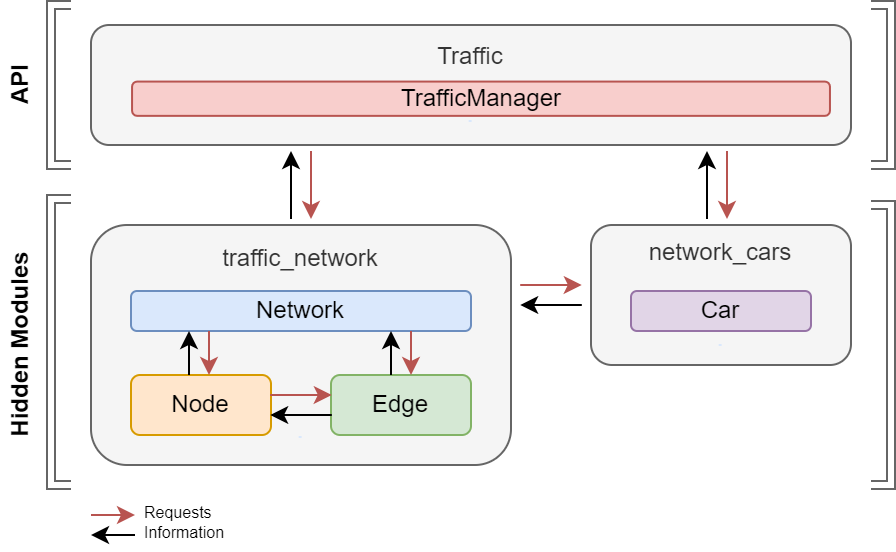
\includegraphics[width=0.9\textwidth]{tex files/Figures/detailed_essentials.png}
	\caption[Software Interaction:  Full View]{Full view of interactions between the modules and their individual components}
	\label{fig:interactions_detailed}
\end{figure}

\noindent  However, as the user doesn't need to concern themselves with the specifics on which functions in which classes work and when, we can streamline the architecture diagram to:

\begin{figure}[H]
    \centering
	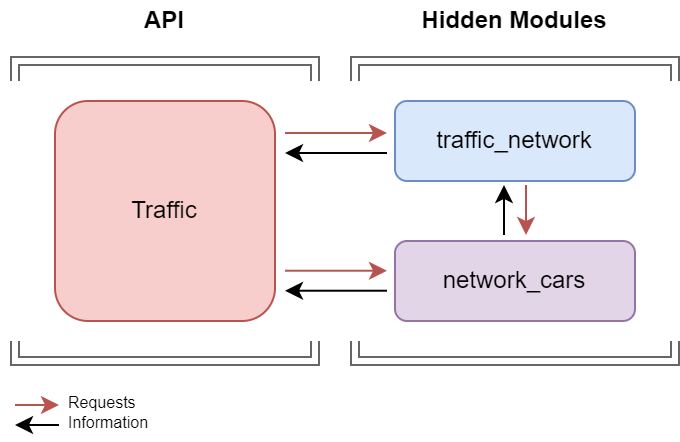
\includegraphics[width=0.7\textwidth]{tex files/Figures/simplified_essentials.png}
	\caption[Software Interaction:  User View]{Generalized overview of interactions between modules}
	\label{fig:interactions_simplified}
\end{figure}



\section{Extended Module Interaction}

Two optional additional modules for generating the underlying network and the car objects themselves can be integrated into the 
% \usetikzlibrary{positioning,matrix,shapes.arrows}

% \tikzset{
%   modulematrix/.style={draw=blue!50!red,rounded corners,matrix of nodes,row sep=1cm,column sep=1cm,nodes={draw=green!70,align=center,font=\sffamily},inner ysep=0.5cm},
%   module/.style={rounded corners, align=center, font=\sffamily, thick},
%   simple module/.style={module, top color=blue!10, bottom color=blue!35, draw=blue!75, text width=40mm, minimum height=15mm},
%   module down arrow/.style={module arrow, shape border rotate=-90},
%   module right arrow/.style={module arrow},
% module arrow/.style={single arrow, single arrow head extend=2.5mm, draw=gray!75, inner color=gray!20, outer color=gray!35, thick, shape border uses incircle, anchor=tail,minimum height=0.7cm},
% }

% \begin{tikzpicture}
% \node [simple module] (mA) {Item-1};
% \matrix[modulematrix,below=of mA,label={[anchor=south]below:Item-2}] (mB) {Item-3 & Item-4 \\};
% \matrix[modulematrix,right=of mB,nodes={text width=5cm,align=center},label={[anchor=north]above:Module C}] (mC) {Item-5 \\ Item-6 \\};
% \matrix[modulematrix,below=of mC,label={[anchor=south]below:Item-9}] (mD) {Item-7 & Item-8 \\};

% \foreach \n in {mA,mC-1-1,mC,mD}
%   \node[module down arrow,below=1mm of \n] {};

% \foreach \n in {mB-1-1,mB,mD-1-1}
%   \node[module right arrow,right=1mm of \n] {};
% \end{tikzpicture}